\section{Overall Discussion of Siamese-based Experiments}
\label{sec:ExperimentsDisucssion}

In light of what we have presented so far, we have to acknowledge that the utilization of \gls{reid} in object tracking is not as useful for any type of object tracker as we had initially hypothesized. Nonetheless, we believe that similarity learning, on which the modern Siamese tracking paradigm itself is based, is of paramount importance to \gls{vot}. Although \gls{reid} relies on similarity learning, the underlying architecture of the tracker needs to be taken into account, which is what explains some of our failures. On the other hand, we have observed an adoption of attention mechanism in various forms during our research, and even in our case it yields promising results.

The first experiment with the external \gls{reid} model failed because of polluted embedding vectors. The objective was to tackle occlusion, but paradoxically, the occlusion in combination with the high tracker confidence was to blame. We showed that it is difficult to determine a point in time before the occlusion arises where the exemplar is sufficiently visible for future \gls{reid}, particularly if the tracker makes predictions with high confidence. As a result, we ended up with object \glspl{bbox} that sometimes did not contain the object of interest at all. But the \gls{siammot} tracker itself is capable of handling short-term occlusion, especially if the object emerges near the location of its last disappearance. Since these situations occur frequently, our approach often interfered with the tracking process. We observed situations where the object re-appeared after a long time far away from the image location where it disappeared and the \gls{reid} assigned a correct ID. On balance, a direct reasoning based on the \gls{reid} has detrimental effects on the \gls{siammot} model.

Conversely, the second experiment attempted to exploit the fact that the \gls{siammot} approach handles the short-term occlusion very well by altering the \gls{nms} phase with a \featurenms{}~\cite{salscheider2020featurenms} algorithm. Moreover, the popular approach of end-to-end architectures spurred the development of the embedding head. The incentive was to introduce joint training to improve feature formation and make the embedding vectors part of the model itself. However, we had not known about all the possible traps related to the inclusion of embeddings with \gls{rpn}-based architectures. Despite our second failed attempt to improve the \gls{siammot} model, we still believe this experiment has a value of its own. It provides corroborating evidence to the recently published paper aimed at ``unfairness'' of \gls{reid} in \gls{mot}~\cite{zhang2021fairmot}. The process of uncovering the design obstacles was similar to the one described in this paper and we fully agree with the authors' conclusions. To summarize, the primary causes of problems are the prioritization of generating proposals before latent space formation, having multiple identities corresponding to one proposal or multiple proposals corresponding to one identity, feature conflict between the detection and the \gls{reid} tasks, and the imbalance of feature dimensions.

Our third experimental approach followed the philosophy of an end-to-end training. The goal remained the same, \ietext{}~, to tackle the occlusion, at least its partial form. Having observed the ramifications of dealing with axis-aligned \glspl{bbox}, we tried to adopt the attention mechanism~\cite{vaswani2017attention}. The endeavor was to teach to model to better delineate the object boundaries when facing partial occlusion. Our initial, custom implementation was successful in an of itself. But the recently published \gls{dsa}~\cite{yu2021dsa} module that was applied to the \gls{sot} Siamese tracking provided a grounding for the additional inclusion of cross-attention, as we only came up with the self-attention part. Thus, we decided to combine our experience with the already proven approach. Besides, we enhanced the \gls{dsa} module with the modulated form of the \glspl{dcnn}. This modification produced $2.6$\% improvement in the \gls{mota} metric (\tabletext{}~\ref{tab:OrigVsDSAScores}). The major advantage of this extension is the consistent improvement of tracking performance with negligible impact on the inference speed. The cost of adopting this easy-to-implement module is a six-fold increase in the \gls{gpu} \gls{vram} consumption during the training. We count the developed \gls{dsa} module as our contribution as it can be applied in practice since it is the inference phase that is the most important. We do acknowledge that the hardware requirements for the model training are higher, but during the test time, an ordinary laptop \gls{gpu} with at least $4$GB of memory can be utilized.

\begin{table}[!t]
    \centering
    \begin{tabular}{llllll}
        \toprule
        \multirow{2}{*}{\textbf{model}} & \multicolumn{5}{l}{\textbf{inference speed [\gls{fps}]}}                                                                     \\
                                        & \textbf{min.}                                            & \textbf{max.} & \textbf{mean} & \textbf{stdev.} & \textbf{median} \\
        \midrule
        original                        & $22.82$                                                  & $29.84$       & $26.49$       & $1.61$          & $26.67$         \\
        \fembmodel{}                    & $10.28$                                                  & $25.72$       & $18.57$       & $4.70$          & $18.28$         \\
        \dsamodel{}                     & $19.06$                                                  & $29.61$       & $24.16$       & $2.67$          & $24.20$         \\
        \bottomrule
    \end{tabular}
    \caption[\gls{dsa} extension inference time comparison]{Comparison of the inference speed of the original \gls{siammot}, \fembmodel{}, and \dsamodel{} versions. The statistics are based on the per-sequence average \gls{fps} values from $56\ 340$ frames spanning across $40$ sequences provided by the \uadetrac{} validation dataset, with an average sequence length of $1408.5$ frames. Our hardware specifications were \usedgpu{} \gls{gpu} and \usedcpu{} \gls{cpu}.}
    \label{tab:InferenceSpeedComparison}
\end{table}

Our three documented Siamese-related experiments utilized the \uadetrac{} dataset. To the best of our knowledge, this dataset is the closest one to the traffic analysis domain with such a high quality of annotations and quantity of frames while using a static camera. Although our implementations and observations turned out to be useful for general object tracking, we continued with this dataset because of its size and the availability of annotations both for training and testing, with the latter being the primary reason.

We contemplated using the \motseventeen{} benchmark dataset (\sectiontext{}~\ref{ssec:DatasetMOT17},~p.~\pageref{ssec:DatasetMOT17}) on which the original \gls{siammot} model was trained and tested so as to directly compare our implementation with the published scores. However, the experiments we conducted would have been impossible to accomplish to such an extent had we relied exclusively on the \motseventeen{} evaluation. This dataset provides seven video sequences aimed at tracking people. Unlike the \uadetrac{} benchmark, the annotations for the test part of the \motseventeen{} are inaccessible. Thus, a validation set has to be produced from the training data. Even though this is a standard practice in machine learning, we could not successfully adopt it because the given seven sequences are significantly different from each other. On top of that, the amount of available data is also unsatisfactory to reliably cross-validate such a complex model. We tried training on six sequences while the remaining one would be used for validation (and repeating for all combinations), but to no avail. A $5$/$2$ split did not work either. The \gls{mota} performance score on the validation set oscillated around $30$\%, which reduced our confidence in the obtained results. Furthermore, we have not seen using the training set of the \motseventeen{} dataset in this fashion. The standard protocol is to train the model on the full training set, and then submit the inference output on the test data to the server for evaluation. But, as demonstrated in \sectiontext{}~\ref{ssec:DSAExperimentalEvaluation}, we would need dozens of evaluation runs. Such attempts would, according to the official rules, result in being banned from the server. Therefore, we had to rely on a dataset that provided annotations for all sequences. Likewise, we had the very same reasons for not using the \kitti{} object tracking dataset (\sectiontext{}~\ref{ssec:DatasetKITTIObjectTracking},~p.~\pageref{ssec:DatasetKITTIObjectTracking}), too.

% ------------------------------------------------------------------------------
\begin{figure}[t]
    \centerline{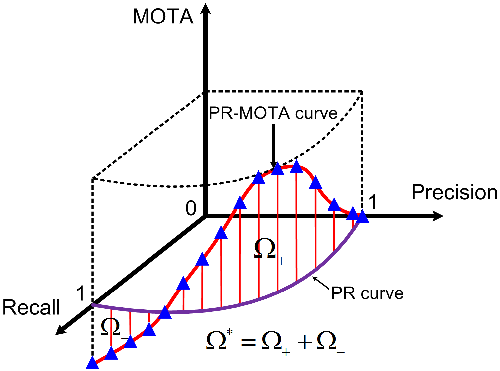
\includegraphics[width=0.5\linewidth]{figures/siamese_tracking/pr_mota_curve.pdf}}
    \caption[Visualization of \gls{mota} along a \gls{pr} curve]{Visualization of the \gls{mota} metric extended to third dimension along a \gls{pr} curve developed as part of the \uadetrac{} benchmark. \externalsrc{\cite{wen2020uadetrac}}}
    \label{fig:PRMOTAVisualization}
\end{figure}
% ------------------------------------------------------------------------------

The \uadetrac{} provides a leaderboard on its own. However, the authors of this dataset proposed new evaluation metrics that are coincidentally inappropriate for our framework, rendering our endeavor to enter the ranking unattainable. They extended the \gls{mota} and \gls{motp} metrics into third dimension by evaluating them along a \gls{pr} curve and then computing an area under the obtained curve (\figtext{}~\ref{fig:PRMOTAVisualization}). We do agree with their justification for introducing another metric as well as the method itself. Nevertheless, the \gls{pr} curve is used to evaluate object detection by altering the threshold value indicating whether a prediction is correct or not. In the case of \gls{siammot}, this is not possible to achieve easily, if at all. Even the official \uadetrac{} leaderboard contains tracking approaches that adopt the ``detection \& linking'' paradigm. In such a setup, the detector itself is an isolated module the output of which is processed by a ``linker'', \egtext{}, some graph-based optimization algorithm. The generation of the \gls{pr} curve is easily produced by altering the threshold over the detector predictions. All it then takes is to run multiple evaluations of the linking phase over several detector predictions. On the other hand, the \gls{siammot} utilizes three threshold values, namely the minimum value for the track to start, to stay active, or to become resumed from a dormant state. Even if we had found a way to emulate the evaluation protocol, we would have done so in an intricate way the credibility of which could be questioned.

Considering this, the use of \gls{clear} metrics (\sectiontext{}~\ref{sec:EvaluatingMOT},~p.~\pageref{sec:EvaluatingMOT}) on top of the \uadetrac{} dataset provided the best combination of traffic-related data with established and widely adopted metrics. After all, the objective was to compare our extensions with the original model in relative terms, and for that our approach served sufficiently.
